


\section{Расчёт координат объектов визуального редактора}


Область редактора представляет собой координатную плоскость,
на которой располагаются компоненты бота.
Расположение компонента обеспечивается координатами $ ( x_k , y_k ) $,
которые указывают
на левый верхний угол компонента.

При перемещении компонента вычисляются смещения
$ \bigtriangleup x $ и $\bigtriangleup y$
относительно координат нажатой мыши
$ (x_m, y_m) $ по формулам
\begin{gather}
	\bigtriangleup x = x_k - x_m, \\
	\bigtriangleup y = y_k - y_m.
\end{gather}

Данные смещения используются для расчёта новых координат компонента
$ (x_k', y_k') $ при перемещении,
которые высчитываются по формулам
\begin{gather}
	x_k' = x_m + \bigtriangleup x, \\
	y_k' = y_m + \bigtriangleup y.
\end{gather}

Расположение компонента на координатной плоскости показано
на рисунке~\ref{f:component-crds}.

\begin{figure}[h]
	\centering
	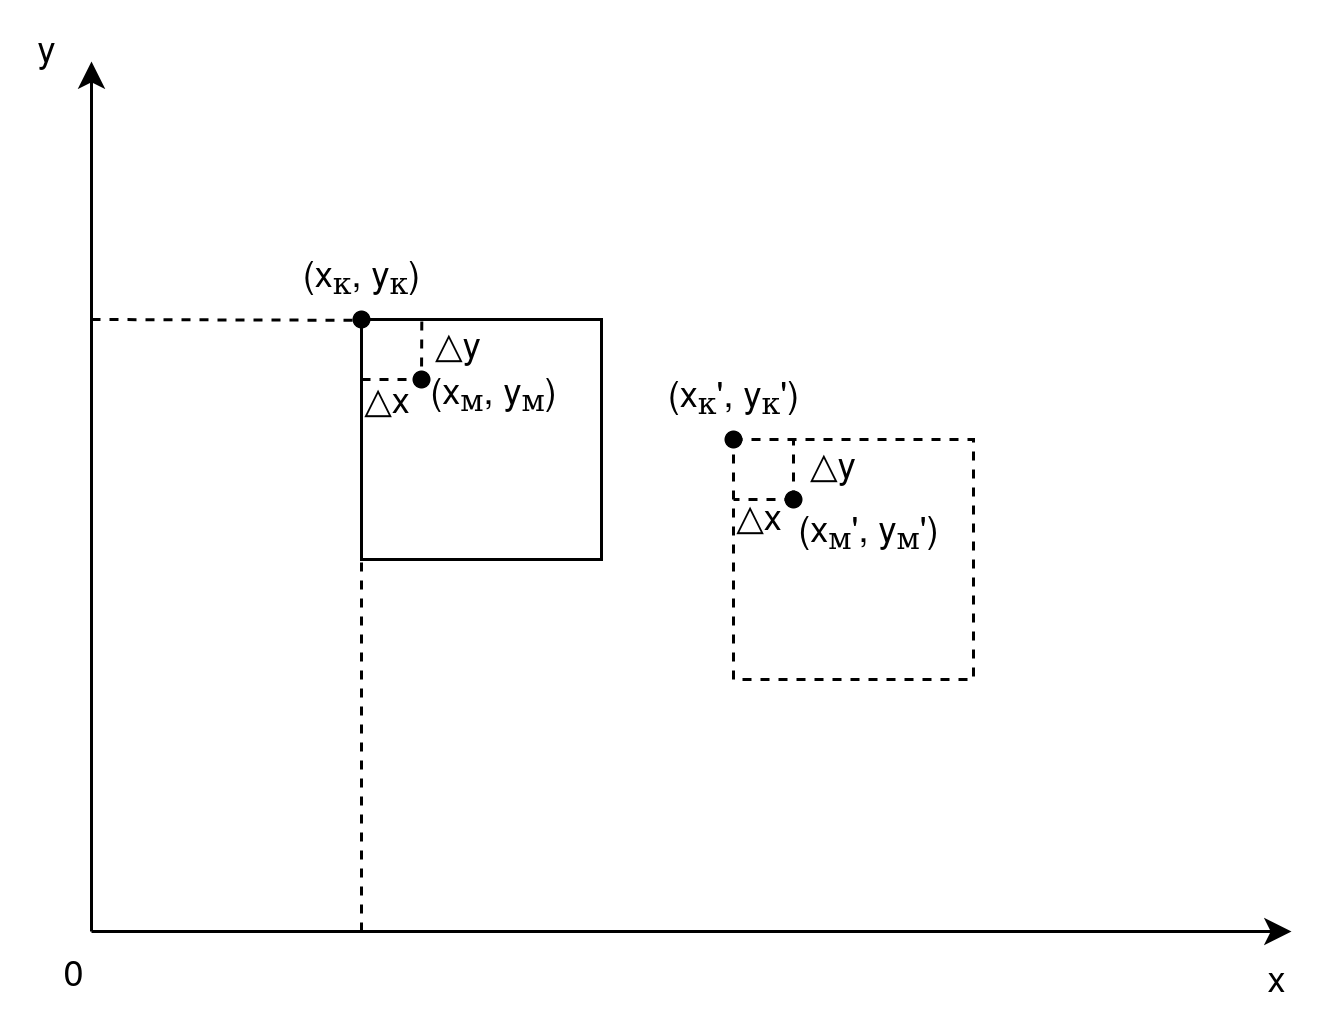
\includegraphics[width=0.7\textwidth]{component-crds}
	\caption{Координаты расположения компонентов}
	\label{f:component-crds}
\end{figure}

Связи между компонентами представляют собой линию со стрелкой.


\begin{figure}[h]
	\centering
	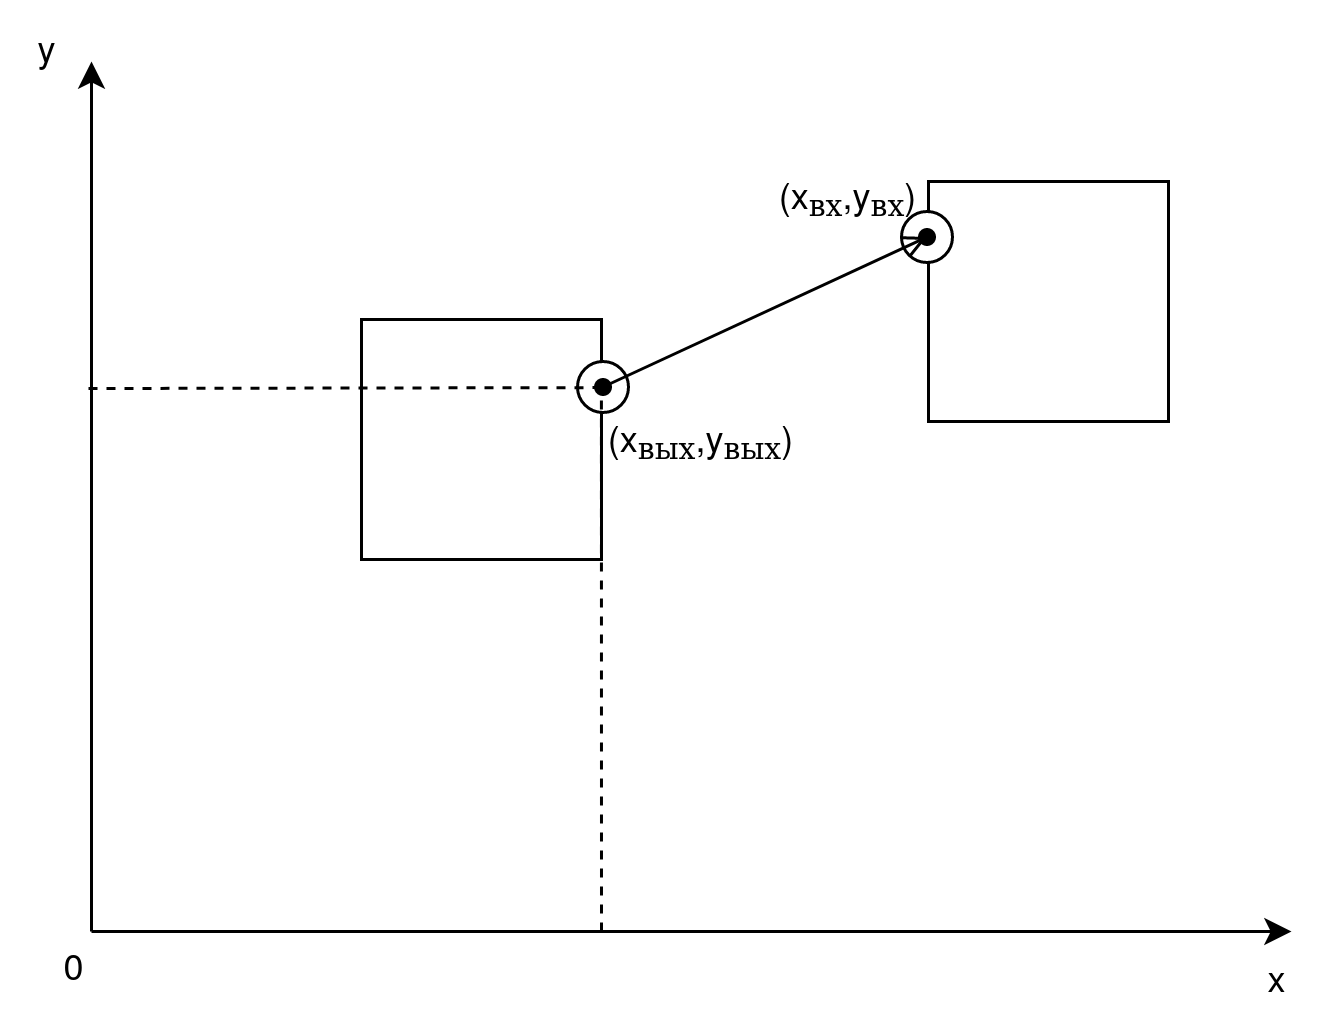
\includegraphics[width=0.7\textwidth]{line-crds}
	\caption{Координаты расположения связей компонентов}
	\label{f:line-crds}
\end{figure}


